\documentclass[11pt,openany,oneside]{book}
\usepackage[a4paper,top=25mm,bottom=23mm,left=25mm,right=22mm,headheight=22pt]{geometry}
\usepackage{fontspec}
\setmainfont{DejaVu Serif}
\setsansfont{DejaVu Sans}
\usepackage{amssymb,xcolor,graphicx,array,booktabs,longtable,tabularx,colortbl,enumitem,tikz,tcolorbox,fancyhdr,titlesec,tocloft,hyperref,eso-pic,microtype,listings}
\usetikzlibrary{arrows.meta,positioning,shapes.geometric,calc}

% Color Palette Definitions
\definecolor{Navy}{HTML}{17365D}
\definecolor{Teal}{HTML}{007F86}
\definecolor{Pale}{HTML}{EAF6F7}
\definecolor{Gold}{HTML}{E3A72F}
\definecolor{Ink}{HTML}{293746}
\definecolor{LightGold}{HTML}{FFF5DD}
\definecolor{SoftGray}{HTML}{F4F6F9}
\definecolor{Coral}{HTML}{D95D50}
\definecolor{Violet}{HTML}{7656A6}
\definecolor{Sky}{HTML}{DCEEFF}
\definecolor{Rose}{HTML}{FCEBE8}

\hypersetup{
    colorlinks=true,
    linkcolor=Teal,
    urlcolor=Teal,
    pdftitle={Web Developer -- Grade XI},
    pdfauthor={Vocational Education Textbook}
}

% List Settings
\setlist[itemize]{leftmargin=1.5em,itemsep=1.5pt,topsep=2pt,parsep=0pt}
\setlist[enumerate]{leftmargin=1.7em,itemsep=2pt,topsep=2pt,parsep=0pt}
\setlength{\parindent}{0pt}
\setlength{\parskip}{3pt}
\setlength{\emergencystretch}{3em}

% Define CSS and JavaScript explicitly; listings does not provide these
% language names consistently across TeX Live installations.
\lstdefinelanguage{CSS}{
  sensitive=true,
  morecomment=[s]{/*}{*/},
  morestring=[b]",
  morestring=[b]',
  alsoletter={-},
  morekeywords={align-items,background,background-color,border,border-radius,box-shadow,
    box-sizing,color,display,flex,font-family,font-size,font-weight,gap,grid-template-columns,
    height,justify-content,margin,max-width,min-height,padding,position,transition,width,
    @media,important,auto,block,grid,none,relative,absolute,center,solid,rem,px,white,black}
}
\lstdefinelanguage{JavaScript}{
  sensitive=true,
  morecomment=[l]{//},
  morecomment=[s]{/*}{*/},
  morestring=[b]",
  morestring=[b]',
  morekeywords={const,let,var,function,return,if,else,for,while,break,continue,
    class,new,this,throw,try,catch,finally,async,await,import,from,export,default,
    true,false,null,undefined,typeof,instanceof,console,log,document,window,
    addEventListener,querySelector,querySelectorAll,getElementById,Math,Number,String,
    Array,Object,Promise,fetch}
}
% Code Listing Style
\lstdefinestyle{webcode}{
    basicstyle=\ttfamily\small,
    keywordstyle=\color{Navy}\bfseries,
    commentstyle=\color{Teal},
    stringstyle=\color{Violet},
    numbers=left,
    numberstyle=\tiny\color{Ink!65},
    stepnumber=1,
    numbersep=8pt,
    showstringspaces=false,
    breaklines=true,
    frame=single,
    rulecolor=\color{Teal!55},
    backgroundcolor=\color{SoftGray},
    xleftmargin=2mm,
    framexleftmargin=2mm,
    aboveskip=5pt,
    belowskip=5pt
}

% Page Border Layout Design
\AddToShipoutPictureBG{
  \begin{tikzpicture}[remember picture,overlay]
    \draw[Navy!65,line width=.55pt] ([xshift=11mm,yshift=-11mm]current page.north west) rectangle ([xshift=-11mm,yshift=11mm]current page.south east);
    \draw[Teal,line width=1.6pt] ([xshift=11mm,yshift=-11mm]current page.north west)--([xshift=37mm,yshift=-11mm]current page.north west);
    \draw[Coral,line width=1.6pt] ([xshift=-11mm,yshift=11mm]current page.south east)--([xshift=-37mm,yshift=11mm]current page.south east);
    \fill[Gold] ([xshift=11mm,yshift=-11mm]current page.north west) circle (1.1mm);
    \fill[Violet] ([xshift=-11mm,yshift=11mm]current page.south east) circle (1.1mm);
  \end{tikzpicture}
}

% Header and Footer Configuration
\pagestyle{fancy}
\fancyhf{}
\fancyhead[L]{\raisebox{-3.5mm}[0pt][0pt]{\small\bfseries\sffamily\color{Teal} WEB DEVELOPER}}
\fancyhead[R]{\raisebox{-3.5mm}[0pt][0pt]{\small\sffamily\color{Navy} GRADE XI TEXTBOOK}}
\fancyfoot[C]{\tikz[baseline=(n.base)]\node[fill=Teal,draw=Gold,line width=.7pt,text=white,circle,minimum size=7mm,inner sep=1pt,font=\small\bfseries] (n) {\thepage};}
\renewcommand{\headrulewidth}{.5pt}
\renewcommand{\headrule}{\hbox to\headwidth{\color{Gold}\leaders\hrule height \headrulewidth\hfill}}

\fancypagestyle{plain}{
  \fancyhf{}
  \fancyhead[L]{\raisebox{-3.5mm}[0pt][0pt]{\small\bfseries\sffamily\color{Teal} WEB DEVELOPER}}
  \fancyhead[R]{\raisebox{-3.5mm}[0pt][0pt]{\small\sffamily\color{Navy} GRADE XI TEXTBOOK}}
  \fancyfoot[C]{\tikz[baseline=(n.base)]\node[fill=Teal,draw=Gold,line width=.7pt,text=white,circle,minimum size=7mm,inner sep=1pt,font=\small\bfseries] (n) {\thepage};}
  \renewcommand{\headrulewidth}{.5pt}
  \renewcommand{\headrule}{\hbox to\headwidth{\color{Gold}\leaders\hrule height \headrulewidth\hfill}}
  \renewcommand{\footrulewidth}{0pt}
}

% Titles Formatting
\titleformat{\chapter}[display]
  {\normalfont\sffamily\bfseries\color{Navy}}
  {\filleft\Large\color{Coral}\chaptername\ \thechapter}
  {.6ex}
  {\color{Teal}\LARGE\raggedright}[\vspace{.5ex}\color{Gold}\rule{\textwidth}{.8pt}]

\titlespacing*{\chapter}{0pt}{-8mm}{.5ex}
\titlespacing*{\section}{0pt}{1.2ex plus .2ex minus .2ex}{.35ex}
\titlespacing*{\subsection}{0pt}{1ex plus .2ex minus .2ex}{.3ex}
\titleformat{\section}{\Large\sffamily\bfseries\color{Teal}}{\color{Coral}\thesection}{.7em}{}
\titleformat{\subsection}{\large\sffamily\bfseries\color{Violet}}{\thesubsection}{.7em}{}

\newcommand{\exampractice}[1]{\begin{tcolorbox}[colback=LightGold,colframe=Gold,boxrule=.6pt,arc=1.2mm,left=2mm,right=2mm,top=1mm,bottom=1mm]\textbf{Review questions.} #1\end{tcolorbox}}
\newcommand{\keyterm}[1]{\textbf{\color{Navy}#1}}

\begin{document}

% Title Page Setup
\begin{titlepage}
\thispagestyle{empty}
\begin{tikzpicture}[remember picture,overlay]
\fill[Navy] (current page.north west) rectangle ([yshift=-11.4cm]current page.north east);
\fill[Teal] ([yshift=-11.4cm]current page.north west) rectangle ([yshift=-11.68cm]current page.north east);
\fill[Coral] ([yshift=-11.68cm]current page.north west) rectangle ([yshift=-11.82cm]current page.north east);
\draw[Gold,line width=2pt] ([xshift=22mm,yshift=-20mm]current page.north west)--([xshift=-22mm,yshift=-20mm]current page.north east);
\draw[Gold,line width=1pt] ([xshift=22mm,yshift=-103mm]current page.north west)--([xshift=-22mm,yshift=-103mm]current page.north east);
\end{tikzpicture}
\vspace*{20mm}{\color{white}\rmfamily\bfseries\fontsize{38}{44}\selectfont HANDBOOK\par}
\vspace{5mm}{\color{Gold}\rule{.72\textwidth}{1.2pt}\par}
\vspace{7mm}{\color{white}\sffamily\LARGE Web Developer\par}
\vspace{3mm}{\color{white}\sffamily\large Grade XI -- IT-ITeS Vocational Education\par}
\vfill
\begin{center}

{\sffamily\Large\bfseries\color{Teal} Web Essentials \textbullet\ HTML \textbullet\ CSS \textbullet\ JavaScript \textbullet\ SDLC\par}
\vspace{4mm}
{\sffamily\large\color{Ink} A structured textbook guide designed for practical web development mastery.\par}
\end{center}
\vfill
\begin{center}{\small Based on Grade XI Web Developer study material topics\par}\end{center}
\end{titlepage}

\frontmatter
\chapter*{About this book}
This handbook covers three foundational pillars of modern web design and client-side web development: Web Development Essentials, HTML/CSS layout systems, and interactive programming using JavaScript. Every section emphasizes practical clarity, clear visual diagrams, real-world examples, and structured review questions.

\tableofcontents
\mainmatter

\chapter*{Module 1. Web Development Essentials}
\addcontentsline{toc}{chapter}{Module 1. Web Development Essentials}

\chapter{Information Technology and ITeS}
\section{Information Technology Overview}
Information Technology (IT) forms the backbone of modern digital operations. It integrates hardware, software networks, databases, human operators, and structured protocols to gather, process, store, and distribute information globally.

\subsection{Key Components}
\begin{itemize}
  \item \textbf{Hardware:} Physical systems, including servers, client workstations, storage arrays, and network interface hardware.
  \item \textbf{Software:} Operating kernels, utility applications, and user frameworks directing hardware behaviors.
  \item \textbf{Networks:} Interconnected hardware links facilitating secure data transport across clients.
  \item \textbf{Data Infrastructure:} Raw data organized efficiently to support analytics, applications, and storage.
\end{itemize}

\section{IT Enabled Services (ITeS)}
ITeS leverages information technology to deliver remote business operations, including customer support, technical assistance, financial processing, and knowledge management.

\begin{center}
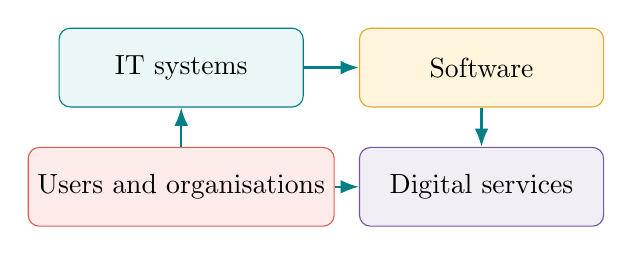
\begin{tikzpicture}[node distance=5mm and 7mm,>=Latex]
\node[draw=Teal,fill=Pale,rounded corners,minimum width=31mm,minimum height=10mm,align=center] (it) {IT systems};
\node[draw=Gold,fill=LightGold,rounded corners,minimum width=31mm,minimum height=10mm,align=center,right=of it] (sw) {Software};
\node[draw=Violet,fill=Violet!10,rounded corners,minimum width=31mm,minimum height=10mm,align=center,below=of sw] (sv) {Digital services};
\node[draw=Coral,fill=Rose,rounded corners,minimum width=31mm,minimum height=10mm,align=center,below=of it] (u) {Users and organisations};
\draw[->,thick,Teal] (it)--(sw);\draw[->,thick,Teal] (sw)--(sv);\draw[->,thick,Teal] (u)--(sv);\draw[->,thick,Teal] (u)--(it);
\end{tikzpicture}
\end{center}
\textit{Figure 1.1.} Interdependence between IT infrastructure and digital user services.

\section*{Review Questions}
\begin{enumerate}
\item Define Information Technology and highlight its primary physical components.
\item Compare voice-based and non-voice business process outsourcing operations.
\item Describe three ways IT infrastructure drives societal growth.
\end{enumerate}

\chapter{Web Design and Development Life Cycle}
\section{Design vs Development}
Web design focuses on visual clarity, branding layout, user experience (UX), and interactive interface structure. Web development constructs the underlying functional codebase using semantic structural markup, declarative styling rules, and execution scripts.

\begin{center}
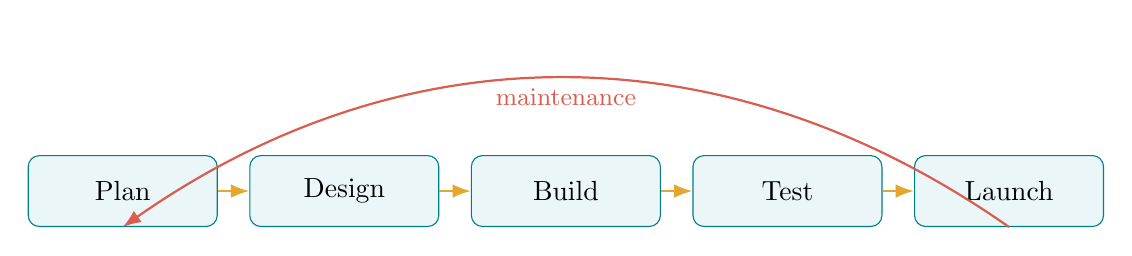
\begin{tikzpicture}[node distance=4mm,>=Latex]
\node[draw=Teal,fill=Pale,rounded corners,minimum width=24mm,minimum height=9mm] (p) {Plan};
\node[draw=Teal,fill=Pale,rounded corners,minimum width=24mm,minimum height=9mm,right=of p] (d) {Design};
\node[draw=Teal,fill=Pale,rounded corners,minimum width=24mm,minimum height=9mm,right=of d] (b) {Build};
\node[draw=Teal,fill=Pale,rounded corners,minimum width=24mm,minimum height=9mm,right=of b] (t) {Test};
\node[draw=Teal,fill=Pale,rounded corners,minimum width=24mm,minimum height=9mm,right=of t] (l) {Launch};
\draw[->,thick,Gold] (p)--(d);\draw[->,thick,Gold] (d)--(b);\draw[->,thick,Gold] (b)--(t);\draw[->,thick,Gold] (t)--(l);
\draw[->,thick,Coral,bend right=35] (l.south) to node[below,font=\small]{maintenance} (p.south);
\end{tikzpicture}
\end{center}
\textit{Figure 2.1.} The iterative cycle of site planning, engineering, and deployment.

\section*{Review Questions}
\begin{enumerate}
\item Explain the key operational differences between web design and software development.
\item Detail why accessibility testing must occur before final deployment.
\end{enumerate}

\chapter*{Module 2. HTML and CSS}
\addcontentsline{toc}{chapter}{Module 2. HTML and CSS}

\chapter{HTML: Document Architecture}
HyperText Markup Language (HTML) provides the fundamental skeletal structure for web content. Elements encapsulate textual data and media objects using semantic tags.

\begin{lstlisting}[style=webcode,language=HTML]
<!DOCTYPE html>
<html lang="en">
<head>
  <meta charset="UTF-8">
  <meta name="viewport" content="width=device-width, initial-scale=1.0">
  <title>Developer Handbook</title>
</head>
<body>
  <header>
    <h1>Web Development Basics</h1>
  </header>
  <main>
    <p>Semantic document structures improve accessibility and indexing.</p>
  </main>
</body>
</html>
\end{lstlisting}

\section*{Review Questions}
\begin{enumerate}
\item What purpose does the \texttt{<!DOCTYPE html>} declaration serve?
\item Write out a basic semantic HTML skeleton including a header, main container, and footer.
\end{enumerate}

\chapter{CSS Layouts and Box Model}
Cascading Style Sheets (CSS) control visual presentation, spacing, typography, colors, and layout positioning across device viewports.

\begin{center}
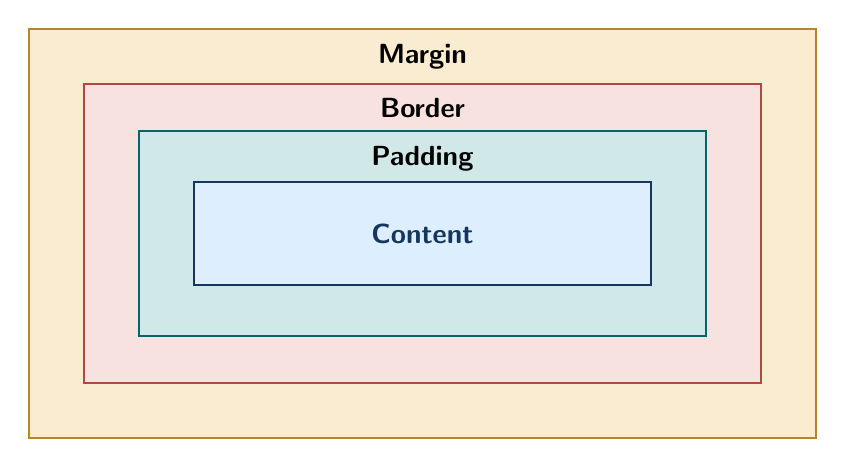
\begin{tikzpicture}
\draw[fill=Gold!22,draw=none] (0,0) rectangle (10,5.2);
\draw[fill=Coral!18,draw=none] (.7,.7) rectangle (9.3,4.5);
\draw[fill=Teal!18,draw=none] (1.4,1.3) rectangle (8.6,3.9);
\draw[fill=Sky,draw=none] (2.1,1.95) rectangle (7.9,3.25);
\draw[Gold!80!black,thick] (0,0) rectangle (10,5.2);
\draw[Coral!80!black,thick] (.7,.7) rectangle (9.3,4.5);
\draw[Teal!80!black,thick] (1.4,1.3) rectangle (8.6,3.9);
\draw[Navy,thick] (2.1,1.95) rectangle (7.9,3.25);
\node[font=\sffamily\bfseries] at (5,4.85) {Margin};
\node[font=\sffamily\bfseries] at (5,4.2) {Border};
\node[font=\sffamily\bfseries] at (5,3.55) {Padding};
\node[font=\sffamily\bfseries\color{Navy}] at (5,2.6) {Content};
\end{tikzpicture}
\end{center}
\textit{Figure 4.1.} Visual layers of the CSS Box Model.

\begin{lstlisting}[style=webcode,language=CSS]
* {
  box-sizing: border-box;
  margin: 0;
  padding: 0;
}
.card {
  width: 100%;
  max-width: 400px;
  padding: 1.5rem;
  border: 1px solid #007F86;
  background-color: #EAF6F7;
}
\end{lstlisting}

\section*{Review Questions}
\begin{enumerate}
\item Describe the four components comprising the CSS Box Model.
\item Explain how \texttt{box-sizing: border-box} simplifies spatial calculations.
\end{enumerate}

\chapter*{Module 3. Web Development Using JavaScript}
\addcontentsline{toc}{chapter}{Module 3. Web Development Using JavaScript}

\chapter{JavaScript Fundamentals}
JavaScript enables dynamic interactive behaviors, state manipulation, event processing, and asynchronous network communication directly within client browser environments.

\begin{center}
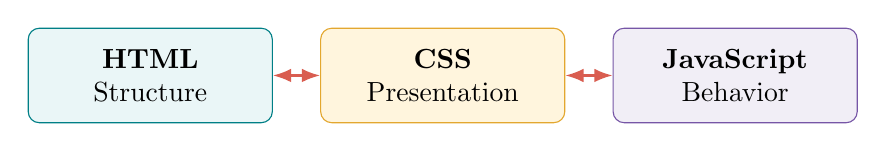
\begin{tikzpicture}[node distance=6mm,>=Latex]
\node[draw=Teal,fill=Pale,rounded corners,minimum width=31mm,minimum height=12mm,align=center] (h) {\textbf{HTML}\\Structure};
\node[draw=Gold,fill=LightGold,rounded corners,minimum width=31mm,minimum height=12mm,align=center,right=of h] (c) {\textbf{CSS}\\Presentation};
\node[draw=Violet,fill=Violet!10,rounded corners,minimum width=31mm,minimum height=12mm,align=center,right=of c] (j) {\textbf{JavaScript}\\Behavior};
\draw[<->,thick,Coral] (h)--(c);\draw[<->,thick,Coral] (c)--(j);
\end{tikzpicture}
\end{center}
\textit{Figure 5.1.} The triad of front-end web development technologies.

\begin{lstlisting}[style=webcode,language=JavaScript]
const calculateTotal = (price, taxRate) => {
  if (price <= 0) {
    throw new Error("Invalid price value provided.");
  }
  return price + (price * taxRate);
};

console.log(calculateTotal(100, 0.18));
\end{lstlisting}

\section*{Review Questions}
\begin{enumerate}
\item Contrast \texttt{let} and \texttt{const} variable scoping rules.
\item Explain how event listeners bind user actions to script logic.
\end{enumerate}



% Additional textbook chapters for a fuller Grade XI learning resource.
\chapter{Requirements, Planning and Project Documents}
\section{Understanding the Need}
A web project begins by understanding the problem it is expected to solve. A website for a school, a small shop, a public service office, and an online learning platform may all use a browser, but each has different users, content, rules, and success measures. Clear requirements prevent avoidable rework and help a team agree on what must be delivered.

\subsection{Stakeholders and Users}
A stakeholder is a person or group affected by the project. Stakeholders may include the customer, website visitors, content editors, administrators, support staff, and the organisation responsible for maintaining the site. Users should be described by their goals rather than by assumptions about their age, device, or technical knowledge.

\subsection{Functional and Non-functional Requirements}
Functional requirements describe what the system must do: display a product catalogue, validate a form, search for an article, or allow an authorised editor to update content. Non-functional requirements describe qualities and constraints, such as response time, accessibility, security, browser support, reliability, and ease of maintenance.

\begin{center}
\begin{tabularx}{\textwidth}{>{\bfseries}p{.24\textwidth}X}
\toprule
Requirement type & Example for a school website\\
\midrule
Functional & A visitor can view announcements and download the academic calendar.\\
Usability & Navigation labels are understandable to first-time visitors.\\
Accessibility & Content can be navigated using a keyboard and read by assistive technology.\\
Performance & Pages avoid unnecessarily large images and scripts.\\
Security & Administrative editing features require authentication.\\
Maintainability & Repeated page elements use consistent templates and styles.\\
\bottomrule
\end{tabularx}
\end{center}

\section{Brief Requirements Document}
A simple project brief should record the purpose, target audience, main pages, required functions, content owner, constraints, and acceptance criteria. Acceptance criteria are observable conditions used to decide whether a feature is complete. For example, “the contact form is finished” is vague; “the form identifies missing required fields and displays a clear confirmation after valid submission” is testable.

\section{Planning and Scope}
Scope defines what is included and what is excluded. A small first release may include a home page, about page, services page, and contact form. A payment system or user account feature may be planned for a later release. A scope list helps the team manage time and avoid adding unplanned work without reviewing its impact.


\section{Business and Software Requirements}
A Business Requirements Document (BRD) describes the business need, intended users, goals, scope, constraints, and expected outcomes. A Software Requirements Specification (SRS) translates the agreed need into detailed system behaviour, interfaces, data requirements, and quality expectations. These documents should be clear enough that a developer can implement the work and a tester can verify it.

A practical BRD may contain the problem statement, project objectives, stakeholders, scope, assumptions, constraints, risks, and acceptance criteria. An SRS may describe functional requirements, non-functional requirements, input and output formats, error handling, external interfaces, and security expectations. For a small classroom project, these can be concise documents rather than lengthy reports.

\section{High-Level and Low-Level Design}
High-level design (HLD) describes the major components of a solution and how they communicate. For a website, it may show the browser interface, application server, database, and external services. Low-level design (LLD) describes the details needed to implement a component, such as field names, validation rules, function responsibilities, or the structure of a page.

\begin{center}
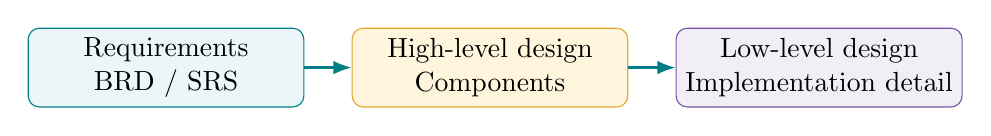
\begin{tikzpicture}[node distance=6mm,>=Latex]
\node[draw=Teal,fill=Pale,rounded corners,minimum width=35mm,minimum height=10mm,align=center] (req) {Requirements\\BRD / SRS};
\node[draw=Gold,fill=LightGold,rounded corners,minimum width=35mm,minimum height=10mm,align=center,right=of req] (hld) {High-level design\\Components};
\node[draw=Violet,fill=Violet!10,rounded corners,minimum width=35mm,minimum height=10mm,align=center,right=of hld] (lld) {Low-level design\\Implementation detail};
\draw[->,thick,Teal] (req)--(hld);
\draw[->,thick,Teal] (hld)--(lld);
\end{tikzpicture}
\end{center}
\textit{Figure 3.1.} Requirements are refined into architecture and implementation detail.

\section{Design Models and Interfaces}
Object-oriented design organises a system around objects that combine data and behaviour. Database design identifies the information that must be stored and the relationships between records. API design defines how separate software components exchange requests and responses. The chosen design should match the project size and should not introduce complexity without a clear need.

\section*{Review Questions}
\begin{enumerate}
\item Distinguish functional requirements from non-functional requirements.
\item Name four stakeholders who may be involved in a website project.
\item Write three acceptance criteria for a school announcements page.
\item Why is it useful to define project scope before coding begins?
\end{enumerate}

\chapter{Web Technologies, Browsers and HTTP}
\section{How a Web Page Reaches a Browser}
When a visitor enters a website address, the browser uses network services to locate the destination server and request resources. The server returns a response, often containing HTML, CSS, JavaScript, images, fonts, or data. The browser interprets these resources and constructs the visible page. This process may involve many requests rather than a single file.

\begin{center}
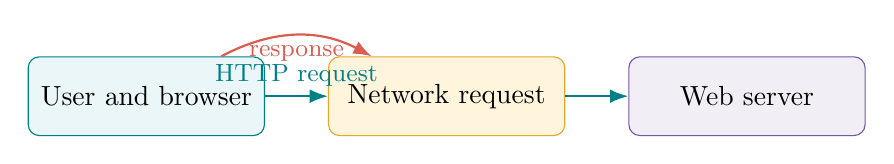
\begin{tikzpicture}[node distance=8mm,>=Latex]
\node[draw=Teal,fill=Pale,rounded corners,minimum width=30mm,minimum height=10mm,align=center] (u) {User and browser};
\node[draw=Gold,fill=LightGold,rounded corners,minimum width=30mm,minimum height=10mm,align=center,right=of u] (n) {Network request};
\node[draw=Violet,fill=Violet!10,rounded corners,minimum width=30mm,minimum height=10mm,align=center,right=of n] (s) {Web server};
\draw[->,thick,Teal] (u)--node[above,font=\small]{HTTP request}(n);
\draw[->,thick,Teal] (n)--(s);
\draw[<-,thick,Coral] (n) to[bend right=28] node[below,font=\small]{response}(u);
\end{tikzpicture}
\end{center}
\textit{Figure 7.1.} A simplified browser-to-server request and response.

\section{HTTP and HTTPS}
HTTP is a protocol used for communication between clients and web servers. A request commonly identifies a method, a resource path, headers, and sometimes a body. A response contains a status code, headers, and usually content. HTTPS protects HTTP communication using TLS, helping protect data from interception or alteration while it travels across the network.

\subsection{Common Status Codes}
\begin{itemize}
\item \textbf{200 OK:} The request was processed successfully.
\item \textbf{301 or 302:} The resource has been redirected.
\item \textbf{400 Bad Request:} The server could not process the request as sent.
\item \textbf{401 Unauthorized:} Authentication is required or has not succeeded.
\item \textbf{403 Forbidden:} The server refuses access to the requested resource.
\item \textbf{404 Not Found:} The requested resource could not be found.
\item \textbf{500 Internal Server Error:} The server encountered an unexpected condition.
\end{itemize}

\section{Browser Developer Tools}
Developer tools help inspect HTML elements, view computed CSS, monitor network requests, read console messages, and test responsive layouts. They are useful for learning because a developer can change a style temporarily, observe the result, and then apply a tested correction to the source code.


\section{Development Tools and Standards}
A web developer commonly uses a code editor, browser, developer tools, image editor, version-control system, and a local testing environment. A code editor helps organise files and detect syntax mistakes; a browser displays the result; developer tools help investigate layout, script, and network problems; and version control records changes so that earlier working versions can be recovered.

HTML, CSS, and JavaScript are interpreted by browsers according to web standards. Consistent indentation, meaningful file names, and a clear folder structure make a project easier to review. A small site might use \texttt{index.html}, \texttt{styles.css}, \texttt{script.js}, and an \texttt{images} folder. Keep source files separate by responsibility unless a particular platform requires another structure.

\section{Common Application Development Models}
The Waterfall model organises work into sequential phases such as requirements, design, implementation, testing, and maintenance. It can be straightforward when requirements are stable, but changes discovered late may be expensive. The Iterative model develops a solution through repeated cycles, refining it after feedback. Agile approaches organise work into small increments and encourage frequent collaboration, review, and adaptation.

No single model is best for every project. A small student website may be planned with a simple checklist and improved after each review. A regulated or large system may need formal documentation and approval steps. The useful question is whether the chosen process helps the team deliver the required quality while responding appropriately to change.

\section*{Review Questions}
\begin{enumerate}
\item Describe the basic request-and-response cycle of a web page.
\item Why is HTTPS preferred when information is sent between a browser and server?
\item Explain the difference between a 404 response and a 500 response.
\item Name three tasks that browser developer tools can support.
\end{enumerate}

\chapter{Semantic HTML and Accessible Structure}
\section{Meaningful HTML Elements}
Semantic HTML uses elements that communicate the role of content. Elements such as \texttt{header}, \texttt{nav}, \texttt{main}, \texttt{article}, \texttt{section}, and \texttt{footer} provide more meaning than using generic containers for every part of a page. Clear structure can improve maintainability and help assistive technologies interpret the document.

\begin{lstlisting}[style=webcode,language=HTML]
<header>
  <h1>Community Learning Centre</h1>
  <nav aria-label="Main navigation">
    <a href="#courses">Courses</a>
    <a href="#contact">Contact</a>
  </nav>
</header>
<main>
  <section id="courses">
    <h2>Available courses</h2>
    <p>Explore the current learning options.</p>
  </section>
</main>
<footer>
  <p>Contact the centre for further information.</p>
</footer>
\end{lstlisting}

\section{Headings and Content Hierarchy}
Headings should describe the topic beneath them and follow a logical hierarchy. A page usually has one main heading, followed by section headings and, where necessary, subheadings. Heading levels should not be selected merely to obtain a desired font size; visual appearance belongs in CSS, while the heading element communicates structure.


\section{Lists and Grouped Information}
HTML supports ordered lists, unordered lists, and description lists. Use an unordered list when the order does not matter, such as a list of required materials. Use an ordered list when the sequence matters, such as installation steps. A description list can pair terms with their explanations.

\begin{lstlisting}[style=webcode,language=HTML]
<h2>Preparation checklist</h2>
<ul>
  <li>Open the code editor.</li>
  <li>Create a project folder.</li>
  <li>Save the first HTML page.</li>
</ul>

<h2>Development sequence</h2>
<ol>
  <li>Plan the page.</li>
  <li>Build the structure.</li>
  <li>Test the result.</li>
</ol>
\end{lstlisting}
Nested lists are useful when a main item has related sub-items, but deep nesting can make information difficult to scan. Choose the list type according to the meaning of the content, not its default appearance.

\section{Links, Images and Alternative Text}
Link text should tell users what will happen when it is selected. Phrases such as “Read the admission requirements” are more informative than repeated “click here” links. Images that communicate information should have concise alternative text. Decorative images can use empty alternative text so that assistive technologies do not announce unnecessary details.

\section{Forms and Labels}
A form control should have a clear label. Placeholder text is not a replacement for a label because it disappears when the user enters a value and may be difficult to read. Required fields should be indicated clearly, and error messages should explain how to correct a problem.

\begin{lstlisting}[style=webcode,language=HTML]
<form>
  <label for="email">Email address</label>
  <input id="email" name="email" type="email" required>
  <button type="submit">Send request</button>
</form>
\end{lstlisting}

\section*{Review Questions}
\begin{enumerate}
\item What is the purpose of semantic HTML?
\item Explain why heading levels should follow a meaningful order.
\item What makes alternative text useful?
\item Why should a form input have an associated label?
\end{enumerate}

\chapter{CSS Selectors, Cascade and Responsive Layout}
\section{Selectors}
CSS selectors identify the elements to which a rule applies. Element selectors target a tag name, class selectors target a reusable class, and ID selectors target an element with a specific identifier. Selectors should be chosen to make styles understandable and easy to maintain.

\begin{lstlisting}[style=webcode,language=CSS]
/* Element selector */
p { line-height: 1.6; }

/* Reusable class selector */
.notice {
  border-left: 4px solid #007F86;
  padding: 1rem;
}

/* Layout for a group of cards */
.card-grid {
  display: grid;
  grid-template-columns: repeat(3, minmax(0, 1fr));
  gap: 1rem;
}
\end{lstlisting}

\section{Cascade, Specificity and Inheritance}
When more than one CSS rule can apply to an element, the cascade determines which declaration wins. Origin, importance, specificity, and source order affect the result. Inherited properties such as text colour may pass from a parent to its children, while properties such as margin do not normally inherit. Overusing highly specific selectors can make future changes difficult.

\section{Responsive Design}
Responsive design helps a layout adapt to different screen sizes. Flexible widths, relative units, CSS Grid, Flexbox, and media queries can be combined to create interfaces that work on phones, tablets, laptops, and larger screens. A responsive page should not merely shrink; content must remain readable and controls must remain usable.

\begin{lstlisting}[style=webcode,language=CSS]
.card-grid {
  display: grid;
  grid-template-columns: repeat(3, minmax(0, 1fr));
  gap: 1rem;
}
@media (max-width: 700px) {
  .card-grid {
    grid-template-columns: 1fr;
  }
}
\end{lstlisting}

\section{Flexbox and Grid}
Flexbox is useful for arranging items along one primary axis, such as a navigation row. Grid is useful when a layout needs rows and columns together, such as a card gallery. Choosing the simpler layout model usually makes the code easier to understand.

\section*{Review Questions}
\begin{enumerate}
\item Compare class selectors and ID selectors.
\item What does CSS specificity help determine?
\item Explain one practical difference between Flexbox and Grid.
\item How can a media query improve mobile usability?
\end{enumerate}

\chapter{JavaScript Variables, Types and Operators}
\section{Storing Values}
Variables give names to values used by a program. JavaScript provides \texttt{const} for bindings that should not be reassigned and \texttt{let} for bindings that may change. \texttt{var} is part of the language but has different scoping behaviour and is usually avoided in new beginner examples.

\begin{lstlisting}[style=webcode,language=JavaScript]
const courseName = "Web Development";
let completedLessons = 3;
completedLessons = completedLessons + 1;

const isReady = completedLessons >= 4;
console.log(courseName, completedLessons, isReady);
\end{lstlisting}

\section{Common Data Types}
Strings represent text, numbers represent numeric values, booleans represent true or false, and arrays hold ordered collections. Objects group related properties. The value \texttt{null} can represent an intentional absence of a value, while \texttt{undefined} commonly indicates that a value has not been assigned or is missing.

\section{Operators and Comparisons}
Arithmetic operators perform calculations. Comparison operators produce Boolean results, and logical operators combine conditions. Strict equality (\texttt{===}) compares values without automatically converting different types, which makes it a good default for most comparisons.

\section{Readable and Safe Code}
Descriptive variable names, consistent indentation, and small expressions make code easier to review. Validate user-provided data before relying on it. Never treat browser-side validation as the only protection for a system that stores sensitive data; server-side checks are also required when a server is involved.

\section*{Review Questions}
\begin{enumerate}
\item Compare \texttt{let} and \texttt{const}.
\item Name four JavaScript data types and give an example of each.
\item Why is strict equality often preferred?
\item Why should important validation not rely only on browser-side code?
\end{enumerate}

\chapter{Conditions, Loops, Functions and Arrays}
\section{Conditional Decisions}
Conditional statements allow a program to choose an action based on a condition. An \texttt{if}/\texttt{else} statement can validate input, choose a message, or control which content is shown. Conditions should be written clearly and tested for both expected and unexpected values.

\begin{lstlisting}[style=webcode,language=JavaScript]
const score = 76;
if (score >= 80) {
  console.log("Excellent");
} else if (score >= 50) {
  console.log("Pass");
} else {
  console.log("Needs more practice");
}
\end{lstlisting}

\section{Loops}
Loops repeat an operation while a condition is true or for each item in a collection. A loop needs a clear stopping condition; otherwise it may continue indefinitely. For arrays, methods such as \texttt{forEach}, \texttt{map}, and \texttt{filter} can express common operations when used appropriately.

\section{Functions}
A function groups instructions into a reusable unit. Parameters receive input, and a return value provides a result. Small functions are easier to test than one long block of mixed responsibilities.

\begin{lstlisting}[style=webcode,language=JavaScript]
function calculateAverage(values) {
  if (values.length === 0) return 0;
  const total = values.reduce((sum, value) => sum + value, 0);
  return total / values.length;
}
console.log(calculateAverage([70, 80, 90]));
\end{lstlisting}

\section{Arrays and Objects}
Arrays are suitable for ordered lists such as course names. Objects are suitable for related attributes such as a course title, duration, and level. Choosing an appropriate data structure reduces repetition and helps the program represent information clearly.


\section{Working with Strings}
A string is a sequence of text characters. JavaScript provides properties and methods for checking length, changing letter case, finding text, extracting a portion, and joining values. String methods usually return a result rather than changing the original string, so store the returned value when a change is needed.

\begin{lstlisting}[style=webcode,language=JavaScript]
const learner = "  Siva Sai  ";
const cleaned = learner.trim();
const greeting = "Welcome, " + cleaned + "!";
console.log(greeting);
console.log(cleaned.toUpperCase());
\end{lstlisting}
When processing names or messages, consider empty input and extra spaces. Do not assume that every text value is valid simply because it is a string; validation should match the purpose of the field.

\section*{Review Questions}
\begin{enumerate}
\item Explain how an \texttt{if}/\texttt{else} statement makes a decision.
\item What is the purpose of a loop's stopping condition?
\item Define function parameters and return values.
\item Give one example of information that is better represented by an object than by separate variables.
\end{enumerate}

\chapter{DOM, Events and Form Interaction}
\section{The Document Object Model}
The Document Object Model (DOM) represents a page as a tree of objects. JavaScript can select elements, read or update text, change classes, and respond to events. Changes should be made deliberately so that the page remains understandable and accessible.

\begin{lstlisting}[style=webcode,language=JavaScript]
const button = document.querySelector("#show-message");
const message = document.querySelector("#message");

button.addEventListener("click", () => {
  message.textContent = "Your action was received.";
});
\end{lstlisting}

\section{Events}
Events describe interactions such as clicks, keyboard input, form submission, and changes to a field. An event listener connects an event to a function. For forms, listening to the submit event makes it possible to validate data before displaying a result or sending a request.

\section{Validation and Feedback}
Good validation explains what needs correction. It should preserve user input where possible, identify the field with an issue, and avoid relying on colour alone to communicate errors. A successful action should also provide clear confirmation.

\section{Safe DOM Updates}


\section{Drawing with the HTML Canvas}
The HTML \texttt{canvas} element provides a drawing surface that JavaScript can control. It is useful for simple charts, sketches, or interactive visual demonstrations. Canvas content is drawn with script and is not automatically exposed as ordinary text to assistive technology; provide a text explanation or an accessible alternative where the drawing conveys important information.

\begin{lstlisting}[style=webcode,language=HTML]
<canvas id="demo-canvas" width="320" height="140">
  A simple coloured rectangle illustration.
</canvas>
\end{lstlisting}

\begin{lstlisting}[style=webcode,language=JavaScript]
const canvas = document.querySelector("#demo-canvas");
const context = canvas.getContext("2d");

context.fillStyle = "#007F86";
context.fillRect(20, 20, 180, 70);
context.fillStyle = "#17365D";
context.font = "16px sans-serif";
context.fillText("Web Developer", 30, 115);
\end{lstlisting}
The canvas dimensions define its drawing surface. CSS can control how large it appears on the page, but changing only its displayed size may scale the drawing. For beginner projects, keep the example small and test it in the browser.
When displaying untrusted text, prefer \texttt{textContent} rather than inserting arbitrary HTML with \texttt{innerHTML}. This reduces the risk of interpreting user input as markup or script. More complex applications need additional security controls appropriate to their data and architecture.


\section{Using JavaScript with Images}
JavaScript can respond to a button click by changing an image's source, updating alternative text, or adjusting presentation classes. Alternative text should continue to describe the image's purpose after a change. Images should have appropriate dimensions and should not be stretched in ways that distort their content.

\begin{lstlisting}[style=webcode,language=HTML]
<img id="course-image"
     src="images/html-basics.jpg"
     alt="HTML code displayed in an editor">
<button id="change-image" type="button">
  Show CSS image
</button>
\end{lstlisting}

\begin{lstlisting}[style=webcode,language=JavaScript]
const image = document.querySelector("#course-image");
const changeButton = document.querySelector("#change-image");

changeButton.addEventListener("click", () => {
  image.src = "images/css-basics.jpg";
  image.alt = "CSS rules displayed in an editor";
});
\end{lstlisting}
The image paths must point to files that actually exist in the project. If an image cannot load, provide a useful fallback or ensure that the page still communicates its essential information.

\section*{Review Questions}
\begin{enumerate}
\item What does the DOM represent?
\item Describe how an event listener works.
\item Give two characteristics of helpful form validation.
\item Why is \texttt{textContent} a safer default for displaying plain user input?
\end{enumerate}

\chapter{Testing, Debugging and Quality Assurance}
\section{Why Testing Matters}
Testing checks whether a website behaves as expected and helps detect defects before release. Testing should cover more than whether a page appears on one developer's computer. Different screen sizes, keyboard use, input errors, navigation paths, and browser behaviours can reveal problems that are otherwise missed.

\subsection{Useful Test Categories}
\begin{itemize}
\item \textbf{Functional testing:} Confirms links, forms, buttons, and core features behave correctly.
\item \textbf{Visual testing:} Checks alignment, spacing, contrast, and layout consistency.
\item \textbf{Responsive testing:} Checks content at narrow and wide viewport sizes.
\item \textbf{Accessibility testing:} Checks keyboard navigation, labels, headings, and alternative text.
\item \textbf{Compatibility testing:} Checks behaviour in supported browsers and devices.
\item \textbf{Regression testing:} Rechecks existing features after a change.
\end{itemize}

\section{A Practical Debugging Method}
First reproduce the issue and record the steps. Next inspect the relevant element, console message, network response, or source code. Form a small hypothesis, change one thing at a time, and repeat the test. Once fixed, check nearby features to make sure the correction did not introduce another defect.

\section{Test Case Example}
\begin{tabularx}{\textwidth}{p{.23\textwidth}X}
\toprule
Field & Example\\
\midrule
Test objective & Verify required email input.\\
Starting condition & Contact form is open.\\
Action & Submit without entering an email address.\\
Expected result & The form identifies the missing required field and does not report a successful submission.\\
Observed result & Record what actually happened.\\
Status & Pass or fail after comparison with the expected result.\\
\bottomrule
\end{tabularx}

\section*{Review Questions}
\begin{enumerate}
\item Why is responsive testing important?
\item Distinguish functional testing from regression testing.
\item List the steps in a systematic debugging process.
\item What information should a useful test case record?
\end{enumerate}

\chapter{Accessibility, Performance and Secure Publishing}
\section{Accessibility Essentials}
Accessible design helps people with different abilities use a website. Provide clear headings, descriptive links, form labels, sufficient colour contrast, keyboard access, and useful alternative text. Interactive controls should show a visible focus indicator. Automated checks can help, but manual keyboard and content checks remain valuable.

\section{Performance Basics}
Large images, unnecessary scripts, repeated network requests, and complex layouts can slow a page. Resize images appropriately, use modern image formats where supported, avoid loading resources that are not needed, and keep code organised. Performance should be evaluated with measurements rather than guesses.

\section{Security Awareness}
Use HTTPS for published sites. Do not place passwords, private API keys, or confidential tokens in public HTML, CSS, JavaScript, or source repositories. Client-side code is visible to visitors. If a feature requires a secret credential, it generally belongs in a protected server-side environment. Keep software dependencies maintained and collect only the information a site actually needs.

\section{Publishing Checklist}
Before publishing, verify that links work, page titles are meaningful, images have suitable alternative text, forms give clear feedback, layouts work on mobile screens, and no test credentials or private data remain in the repository. Confirm the correct files are deployed and keep a copy of the source so that later updates can be made safely.

\section*{Review Questions}
\begin{enumerate}
\item List five practices that improve accessibility.
\item Name three common causes of slow web pages.
\item Why should secret API keys not be stored in browser-side JavaScript?
\item Create a short checklist for publishing a small informational website.
\end{enumerate}

\chapter{Integrated Mini Project: Learning Centre Website}
\section{Project Brief}
Create a small informational website for a learning centre. The website should display the centre name, a list of courses, basic contact information, and a contact form interface. The project demonstrates the combined roles of HTML for structure, CSS for presentation, and JavaScript for interaction.

\section{Suggested Page Structure}
\begin{itemize}
\item Header containing the site name and primary navigation.
\item Main section describing the centre and its courses.
\item Course cards with titles, brief descriptions, and duration.
\item Contact section with labelled form fields.
\item Footer containing non-sensitive contact and copyright information.
\end{itemize}

\section{Implementation Plan}
Begin by creating semantic HTML. Add CSS rules for typography, colour, spacing, and a responsive card layout. Add JavaScript only where it improves the user experience, such as providing a clear message after a valid client-side form submission. If the project is later connected to a real service, server-side validation and secure handling of submitted information will be required.

\section{Evaluation Rubric}
\begin{tabularx}{\textwidth}{p{.52\textwidth}r}
\toprule
Criterion & Marks\\
\midrule
Semantic structure and meaningful headings & 20\\
Readable and consistent visual design & 20\\
Responsive layout & 20\\
Working interaction and useful feedback & 15\\
Accessibility checks & 15\\
Code organisation and testing notes & 10\\
\midrule
Total & 100\\
\bottomrule
\end{tabularx}

\section*{Review Questions}
\begin{enumerate}
\item Identify the HTML, CSS, and JavaScript responsibilities in the project.
\item Describe how you would test the site on a narrow mobile screen.
\item What security changes would be required before collecting real contact details?
\item Suggest two improvements that could be included in a future version.
\end{enumerate}

\chapter*{Glossary and Quick Revision}
\addcontentsline{toc}{chapter}{Glossary and Quick Revision}
\begin{description}[leftmargin=3.2cm,style=nextline]
\item[Accessibility] Designing and building digital content so that people with varied abilities can use it.
\item[API] A defined way for software components to communicate.
\item[Browser] Software that requests and displays web resources.
\item[CSS] A language used to style and lay out web documents.
\item[DOM] An object representation of a document that scripts can inspect and modify.
\item[HTML] The markup language used to structure web content.
\item[HTTP/HTTPS] Protocols for web communication, with HTTPS protecting the connection using TLS.
\item[JavaScript] A programming language commonly used to add behaviour to web pages.
\item[Responsive design] A design approach that adapts content and layout to different viewport sizes.
\item[Semantic HTML] Markup whose elements describe the role and meaning of content.
\item[Server] A system that responds to requests from clients.
\item[Testing] A process for checking software behaviour against expected results.
\end{description}

\section*{Final Revision Questions}
\begin{enumerate}
\item Explain the relationship between HTML, CSS, and JavaScript.
\item Describe the main stages of a website development life cycle.
\item Compare a functional requirement with a non-functional requirement.
\item Explain how the browser and server communicate using HTTP.
\item Describe semantic HTML and name four semantic elements.
\item Explain the CSS box model and responsive design.
\item Give examples of JavaScript variables, conditions, functions, and arrays.
\item Describe how the DOM and event listeners support interaction.
\item Outline a practical method for testing and debugging a website.
\item List key accessibility, performance, and security checks before publishing.
\end{enumerate}

\end{document}
